
\chapter{Models of Pyramidal Neurons}
\label{chap:pyramidal-neurons}
 
The pyramid shaped cell body, or soma, contains voltage activated sodium and
potassium channels somewhat similar to those studied by Hodgkin and Huxley in
the giant axon of the squid.

Pyramidal neurons receive tens of thousands of synaptic inputs on their
dendrites. Post-synaptic potentials produced in the dendrites can propagate to
the soma to trigger action potentials. Throughout the cell, we also have passive
channels that remain partly open all the time, leading to a leakage resistance.

We model it piece by piece. The usual approach is to model this with a lumped
parameter model in which we divide the neuron into a finite number of
compartments containing resistances, capacitances and batteries to represent
ionic equilibrium potentials. We model this complex neuron with something like
this, Fig.\ref{fig:compartment_neuron}.

\begin{figure}[hbt]
  \centerline{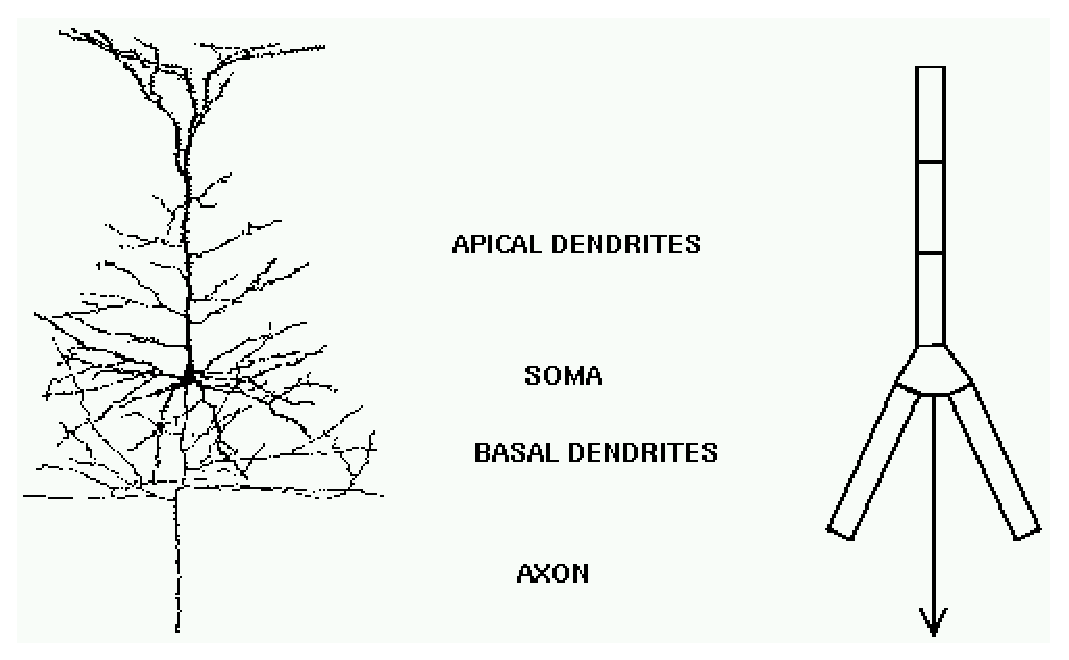
\includegraphics[height=5cm,
    angle=0]{./images/compartment_neuron.eps}}
\caption{A simple representation of the pyrymidal cell}
\label{fig:compartment_neuron}
\end{figure}

Considerable recent evidence indicates that action potentials are often
initiated near the soma rather than at the site of synaptic input in the
dendrites, suggesting that the axon has a low threshold for action potential
initiation.
The mechanism underlying this low threshold has long been assumed to be a high
density of Na+ channels in the axon hillock or initial segment.
However, applying TTX at such sites does not alter the spiking generation. This
suggests that the spiking initiation site is not near the soma; but a a certain
distance. Indeed, application of tetrodotoxin to the axon beyond the initial
segment raises the threshold by 7-10 mV. These results indicate that Na+
channels in the axon (i.e. axonal initiation site - AIS) proper rather than in
the initial segment may determine the threshold.

The low threshold for spiking initiation at such site can be explained by
(require further investigation) - Sect.\ref{sec:NaT-Colbert-2002}
\begin{itemize}
  \item higher $\na$ channel density
  
  \item different electrophysiological properties, e.g. $\na$ channels at AIS
  has more negative half-activation voltage, and probably also less expression
  of $\K$ channels
\end{itemize}



 
\section{Introduction}
\label{sec:introduction-4}

% In the previous chapters of this part, we have studied a nerve cell by
% modelling its parts separately. In this chapter, we will study models
% examining neurons as a whole.
\begin{table}[!hbt]
  \begin{center}
    \caption{Estimate number of pyramidal or granule cells in various
      hippocampal regions}
    \begin{tabular}{cccc} 
      \hline
      Species & Age & Region & Estimate \\ 
      \hline\hline
      Rat & 1 month & CA1 & 320,000-420,000 \\
      & 1month & CA3 & 210,000-330,000 \\
      & adult & CA1-3 & 260,000 \\
      Human & adult & CA2-3 & 2,350,000 \\
      & & CA1 & 4,630,000 \\
    \end{tabular}
  \end{center}
  \label{tab:pyramidal_cell_estimate}
\end{table}
Table \ref{tab:pyramidal_cell_estimate} lists the number of cells in
the hippocampus {\it in vivo}. The number of cells {\it in vitro} is
an order of magnitude smaller, e.g. longitudinal CA3 slice (400$\mu$
thick and 10 nm long) has 20,000 pyramidal cells, and transverse CA3
slice has 3,000-5,000 cells. 

{\bf Experimental approach}: Prepare {\it in vitro} brain slices,
e.g. hippocampal CA3 region with 1,000-20,000 neurons (which is still
small compared to entire hippocampus of order 1million neurons), as
shown in Table~\ref{tab:pyramidal_cell_estimate}. This {\it in vitro}
CA1-3 region, however, can produce different population activities.
Then the data is recorded at different level of organization
\begin{itemize}
\item single neurons within brain slices
\item synaptic interaction between neurons within a slice
\item response of population of neurons under a localized stimulus. 
\end{itemize}

{\bf The reason for using a portion of the brain, rather than
  combining different types of neuronal cells}
\begin{enumerate}
\item such general models, though can be analyzable, and practical in
  engineering applications, do not intended to represent in detail
  actual networks of neurons within a brain
\item using a portion of the brain, experiments are feasible. 
\item hippocampal slice is of anatomical simplicity and technical
  advantage of the system (e.g. relatively straightforward function).
\end{enumerate}

{\bf What's the difference between a model of cortex and models of
invertebrate?}
\begin{enumerate}
\item In invertebrate, many of the neuron possess individual
  identities and distinctive physiological properties, and thus can be
  studied separately 
\item In cortex, the variation are too large that it's impossible to
  study each one as individual. Thus, the properties of hippocampal
  pyramidal cells are properties of a ``generic'' pyramidal cell. In
  other words, the model is not targeted to any particular cell, but
  an ``average'' of the cells in the whole network. 
\end{enumerate}

{\bf Approach for ``generic'' pyramidal cell?}
\begin{enumerate}
\item One way to model interconnected networks of neurons is that all
  neurons of a given type are ``lumped'' into a single representative
  neuron. Thus, the distributed circuitry is compressed into a small
  network, which is hoped still being able to capture the essential
  global behaviors.
  \textcolor{red}{Unfortunately, the lumping approach is not
    applicable to CA3 region. The lumping procedure is not a robust
    approximation of the system.}
\item In hippocampus, it's important to build a separate model for
  each neuron, each with its synaptic connection explicitly to other
  neurons.
\end{enumerate}

{\bf Types of cells in CA3 region}: 90\% of cells in CA3 region are
pyramidal cells (whose synapses are excitatory). Most of the remainder
are inhibitory and use GABA as their neuron transmitter.  The
classification of theses cells are not completed, with different
firing behaviors, postsynaptic actions. However, pyramidal cells are
of the main concern.  Pyramidal cells can be found in hippocampus,
neocortex, and cortical-thalamus. Thus, there can be three different
aims to model.

The pyramidal cell has a small soma and two segregated dendritic
systems. It has a relatively simple cellular architecture and
remarkably constant throughout the mammalian series. The pyramidal
cells are clustered in a compact layer, sending their axons into the
alveus, fimbria and fornix~\citep{kandel1961ehn_a}. 

{\bf Properties of a pyramidal cell}
\begin{enumerate}

\item input resistance (Sect.\ref{sec:input-resistance}) in the slices range
from 20-over 50 M$\Omega$

\item membrane time constant 30-50ms
\item cells can fire not only a single, but a burst of up to 8
  (calcium) spikes at an interval 5-10ms.
  \textcolor{red}{Burst occur both {\it in vivo} and {\it in vitro},
    which is considered an intrinsic property of pyramidal cells}, not
    the result of the hippocampal circuitry.

\end{enumerate}
However, not all CA3 stratum pyramidal cells are burst-firing. They
concentrate in CA3a region which is closed to CA2 than in CA3b
cells.


{\bf Roles of ionic currents to bursting?}:
\begin{enumerate}
\item Burst depend on at least one calcium currents. The block of
  calcium current prevent typical bursting, yet still allowing
  individual action potential (AP) to occur. The diverse shape of
  calcium spike suggest they are initiated at diverse dendritic
  location, i.e.
  \textcolor{red}{there are multiple dendritic sites, each capable of
    generating sodium or calcium spikes or both}

\item It appears that both soma and dendrite of CA3 pyramidal cells
  can generate burst; yet in CA1 pyramidal cells have different
  properties:
  \begin{itemize}
  \item brief injected current in the dendrite or after orthodromic
    stimulation with inhibition blocked can lead to dendritic burst
  \item steady injected current in the soma usually lead to repetitive
    firing, rather than a burst.
  \end{itemize}

\item A burst is terminated by a slow, intrinsic hyperpolarizing
  afterpotential (AHP) mediated by one or more calcium-dependent
  \ce{K+} currents which increase the input conductance of the cells
  by 25-40\%.
  \textcolor{red}{Thus this $I_{AHP}$ is quite complex (we will
    discuss them in each model)}.
\end{enumerate}


A representation of a neuron along with its connections is given in
Fig.~\ref{fig:neuron}. Earliest theoretical results relating the time
course of synaptic potential to the time course of nonuniformly
distributed synaptic current was introduced by Wilfrid Rall since
1957~\footnote{\url{http://www.scholarpedia.org/article/Rall_model}}. It
has been described in Chap.~\ref{sec:ralls-model}.

\begin{figure}[hbt]
  \centerline{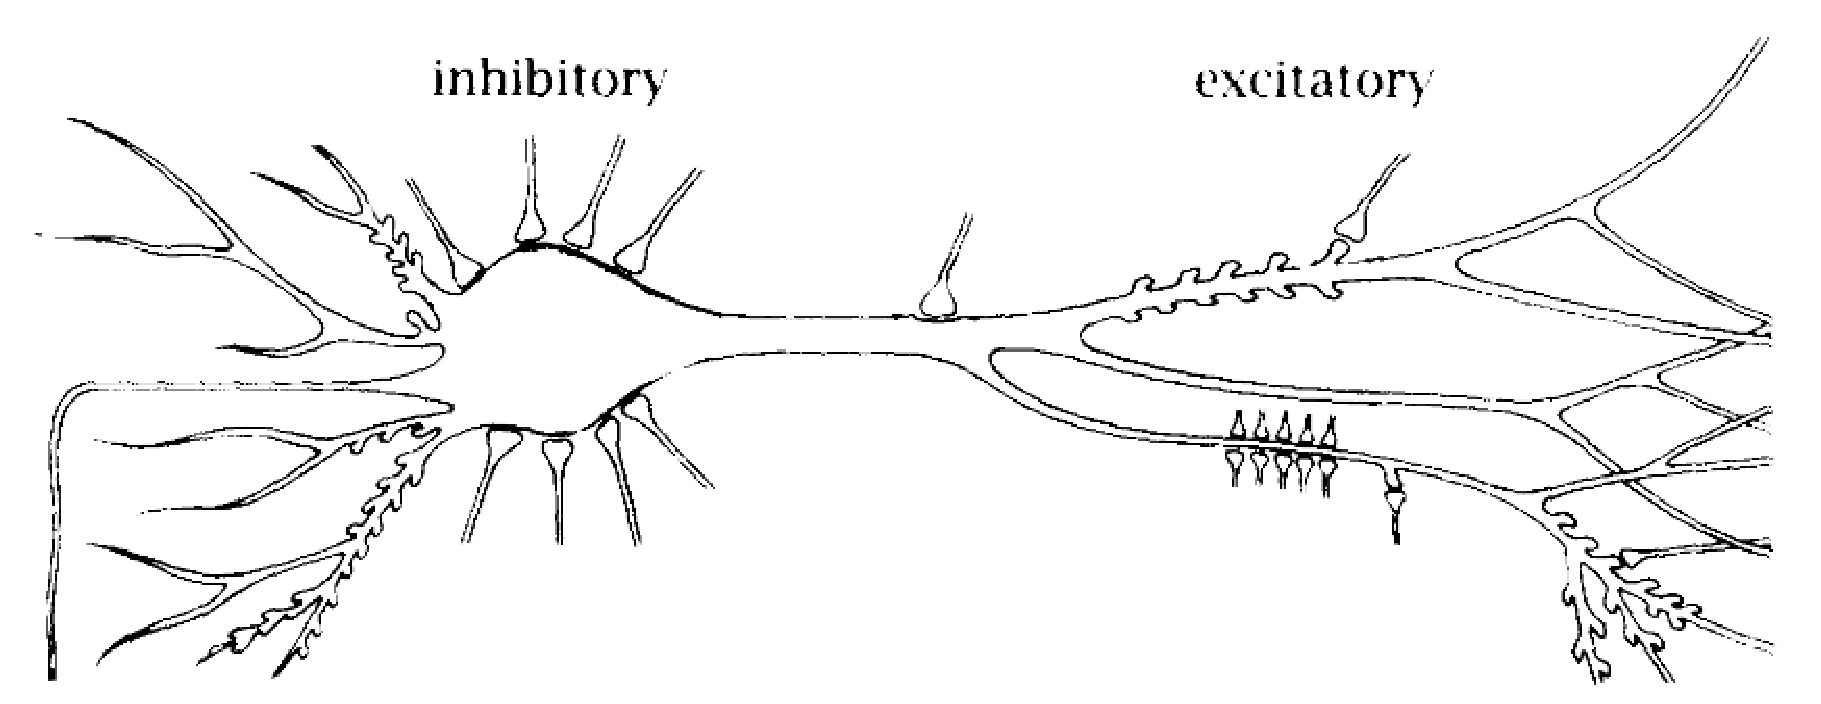
\includegraphics[height=5cm,
    angle=0]{./images/neuron.eps}}
  \caption{Diagram of a CNS neuron with synaptic inputs}
  \label{fig:neuron}
\end{figure}


One of the widely geometrical shape approximated by some parts of the
neurons is cylinder. This cylinder has a conductive core surrounded by
an outer shell or membrane that has different electrical properties
from its core. The currents flow down the center and across the side
of the cylinder. This representation is called {\bf core conductor} or
electrical cable and theory upon which the mathematical models are
built is called {\bf linear cable theory}.

\section{Traub-Llinas (1979) - pyramidal in CA1 hippocampus}
\label{sec:Traub-Llinas-1979}

Rall (1967) has proposed a theoretical model for a 10-compartment
lumped-soma neuron working under subthreshold condition
(sect.~\ref{sec:ralls-model}). 

In 1979, Traub and Llinas developed a model for hippocampal pyramidal cell
(HPC), primarily for CA1 cells~\citep{traub1979hpc} and was partly in analogy
to Purkinje cells.
\begin{enumerate}

  \item  \textcolor{blue}{Dendritic spines has not been considered in the model}.

  \item $g_{Ca}$ was assumed to be in dendritic regions only and 
  
  \item $g_\K$ : located in somatic region. 
  
  \item $g_\na$ is in somatic region, and is localized to certain isolated
  dendritic membrane regions (sodium hot-spot).

\end{enumerate}

In this model, bursts can only be initiated in the soma. \footnote{A burst, as
recorded in CA3 cells, is a train of 2-10 fast sodium-mediated APs and terminate
in one (or sometimes more) slow calcium-mediated spikes.} and can not be
generated without interaction between spatially separated regions.

At the end of a burst, the membrane potential repolarize and then hyperpolarize
- a process known as afterhyperpolarization (AHP)
- Sect.\ref{sec:ahp-after-hyperp} - and last for hundreds of ms, before another
spike can be initiated.

\section{Traub (1982) - pyramidal in CA3 hippocampus in adult
  guinea pig}
\label{sec:Traub-1982}

With the fact that, in CA3 nerve cells, burst can be generated locally and
independently between soma and dendrite, Traub (1982) redesign the bursting
mechanism (compared to the previous work - Sect.\ref{sec:Traub-Llinas-1979}) by
adding all required conductance to generate a burst and its associated long AHP
into every compartment ~\citep{traub1982sib}.
\begin{enumerate}
  \item $g_\na$
  \item $g_\ca$
  
  \item $g_\k$
  \item $g_{\k(\ca)}$
\end{enumerate}
Kinetics were inferred from current-clamp recording
(Sect.\ref{sec:current-clamp-protocol}).

Model's assumption for producing burst
\begin{enumerate}
  \item rapid inactivation of $g_\ca$ (10s of ms) by intracellular $[\Ca]$

This is later considered a wrong assumption.
  
  \item $\Vm$-dependent inactivation of $g_\k$
\end{enumerate}

Model's PROS and CONS:
\begin{itemize}

  \item burst morphologies depend on the region of the cell; and 
  
  \item frequency of burst increases with progressive depolarization
  
  \item the model doesn't switch from repetitive bursting to repetitive spiking
  (i.e. single action-potentials) with further depolarization
  
This result is wrong as it is in contrast to CA3 pyramidal recorded data {\it in
vitro}~\citep{wong1981agh}.

  \item In addition, when incorporated into a networks, it doesn't generate the
  synchronized multiple bursts observed in slices bathing in GABA$_A$ blocker
  picrotoxin.

\end{itemize}

The questions of interest are :
\begin{itemize}
\item why and how a neuron can switch from one firing-pattern mode to
  another?
\item what neuronal properties might be critical to the generation of
  synchronized multiple bursts in a population of cells.
\end{itemize}

\section{Traub (1991) - pyramidal neuron in hippocampus}
\label{sec:Traub-1991}

GOAL: Build a model in that CA3 and CA1 types of firing behavior can be
reproduced by proper manipulation of the membrane conductance densities.

Thanks to
\begin{itemize}
\item whole-cell recording from isolated cell preparation: a more
  precise characterization of many voltage-dependent currents can be
  computed
\item calcium-imaging studies revealed that $g_{Ca}$ widely spreads
  over the cell. 
\end{itemize}

Traub et al.~\citep{traub1991ca3} developed a model for CA3 hippocampal neuron
with 19 compartments (8 for the basal dendrites, 1 for the soma, and 10 for the
apical dendrites); but \textcolor{red}{no branching}. 

Each compartment in Traub's model has a capacitance, a leak conductance, and a
variety of ionic conductances (i.e. 6 active conductances $g_{\ce{Na}},
g_{\ce{Ca}}, g_{K(A)}, g_{\ce{K(Ca)}},$ $ g_{\ce{K(AHP)}},$ $g_{\ce{K(DR)}}$),
with the distribution of maximal conductances shown in
Fig.~\ref{fig:traub_ion_distribution}.
\textcolor{red}{Each distinct compartment is able to generate a burst and its
associated long after-hyperpolarization (AHP)}.

\begin{figure}[hbt]
  \centerline{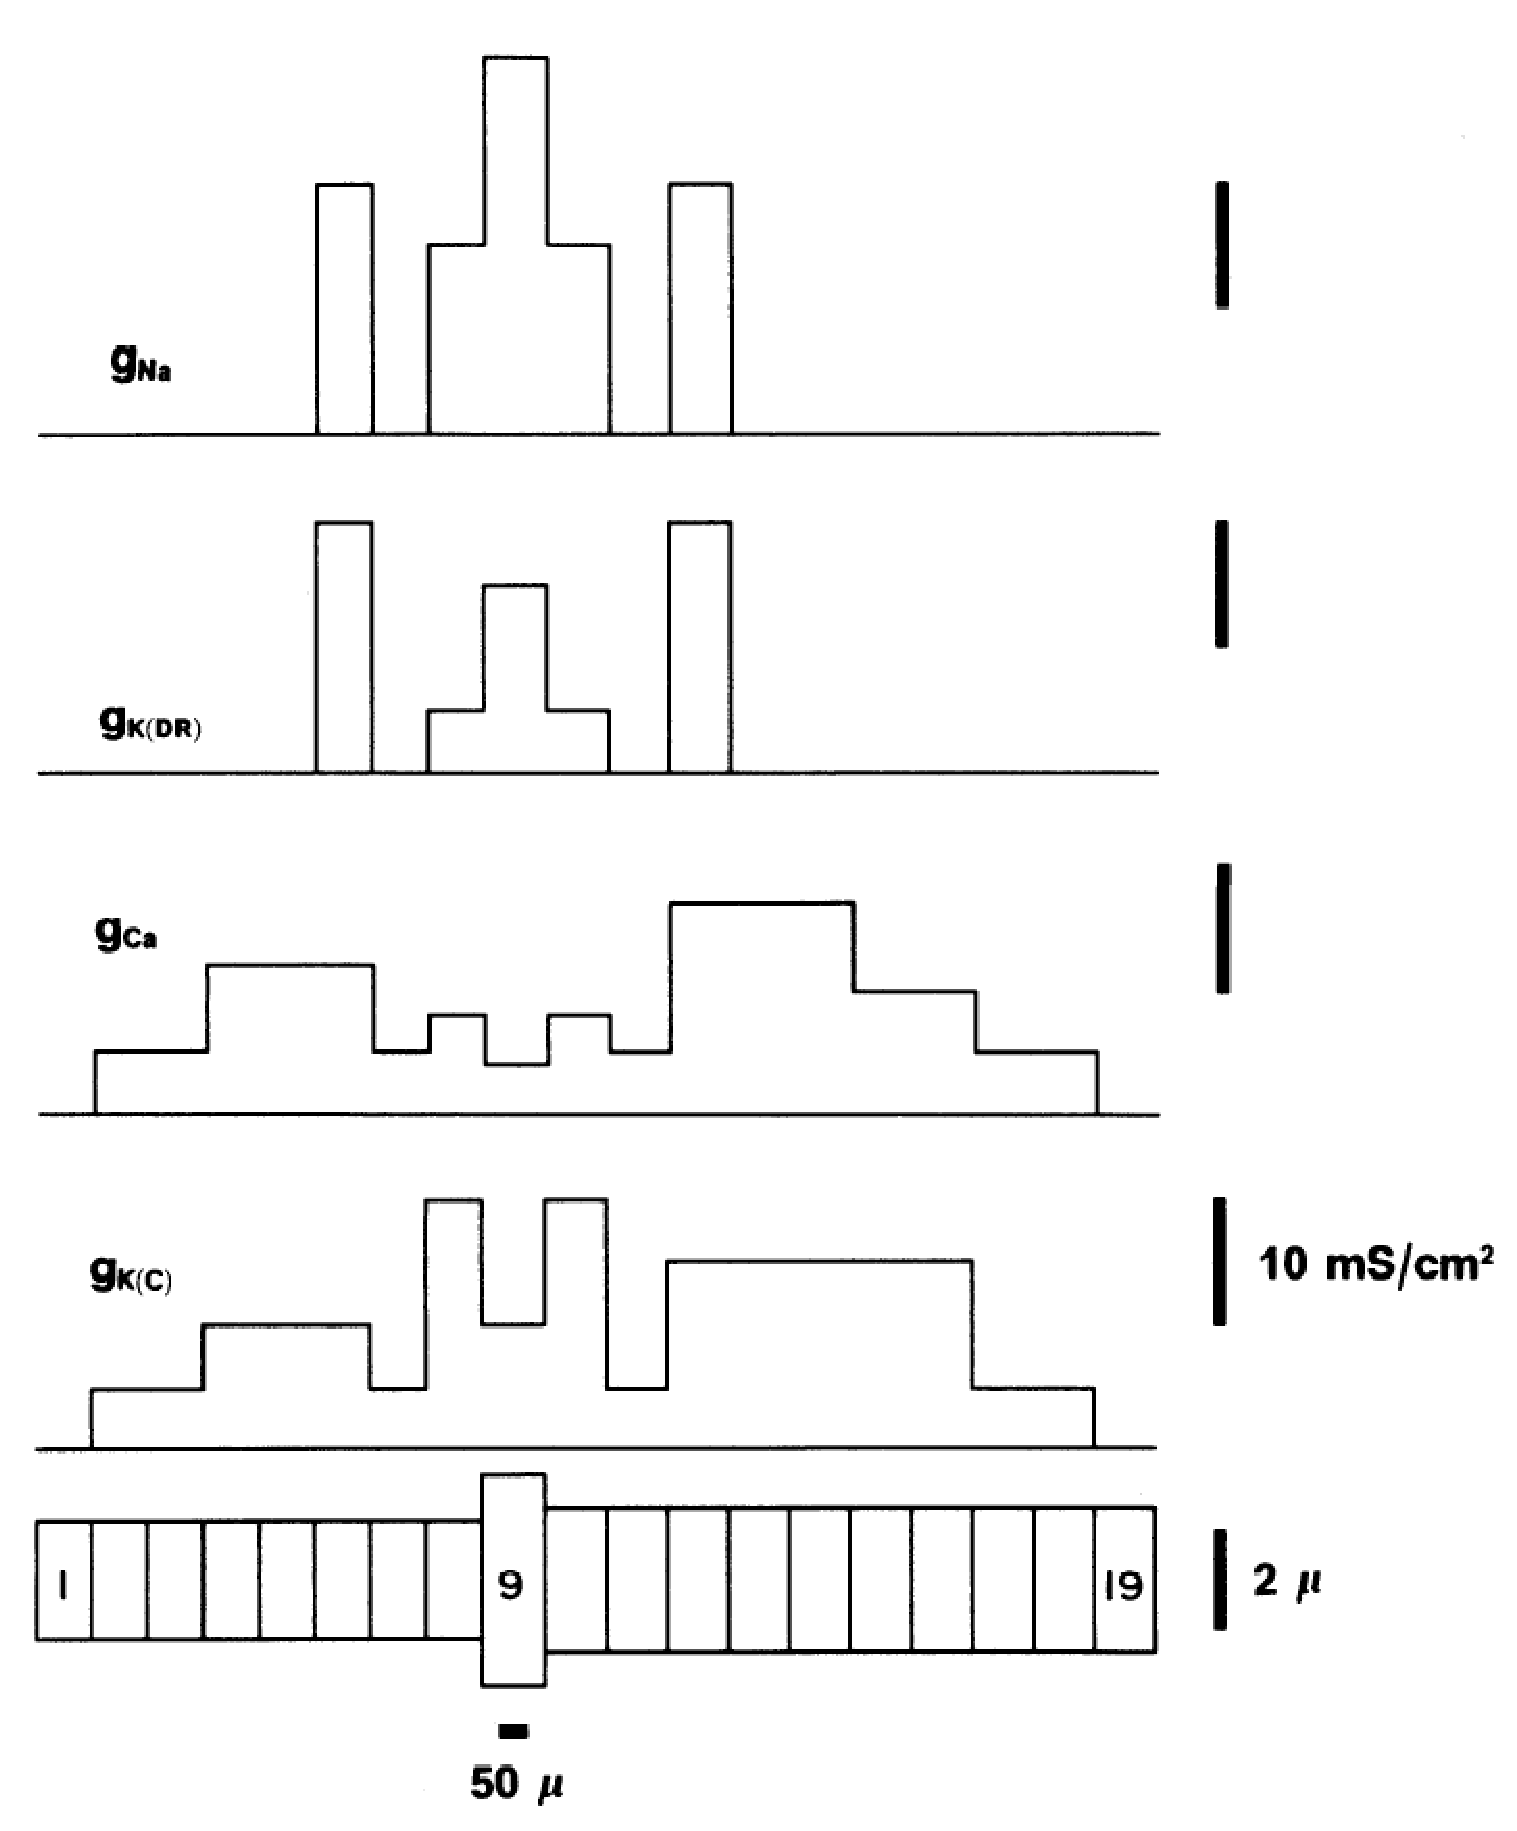
\includegraphics[height=7cm,
    angle=0]{./images/traub_ion_distribution.eps}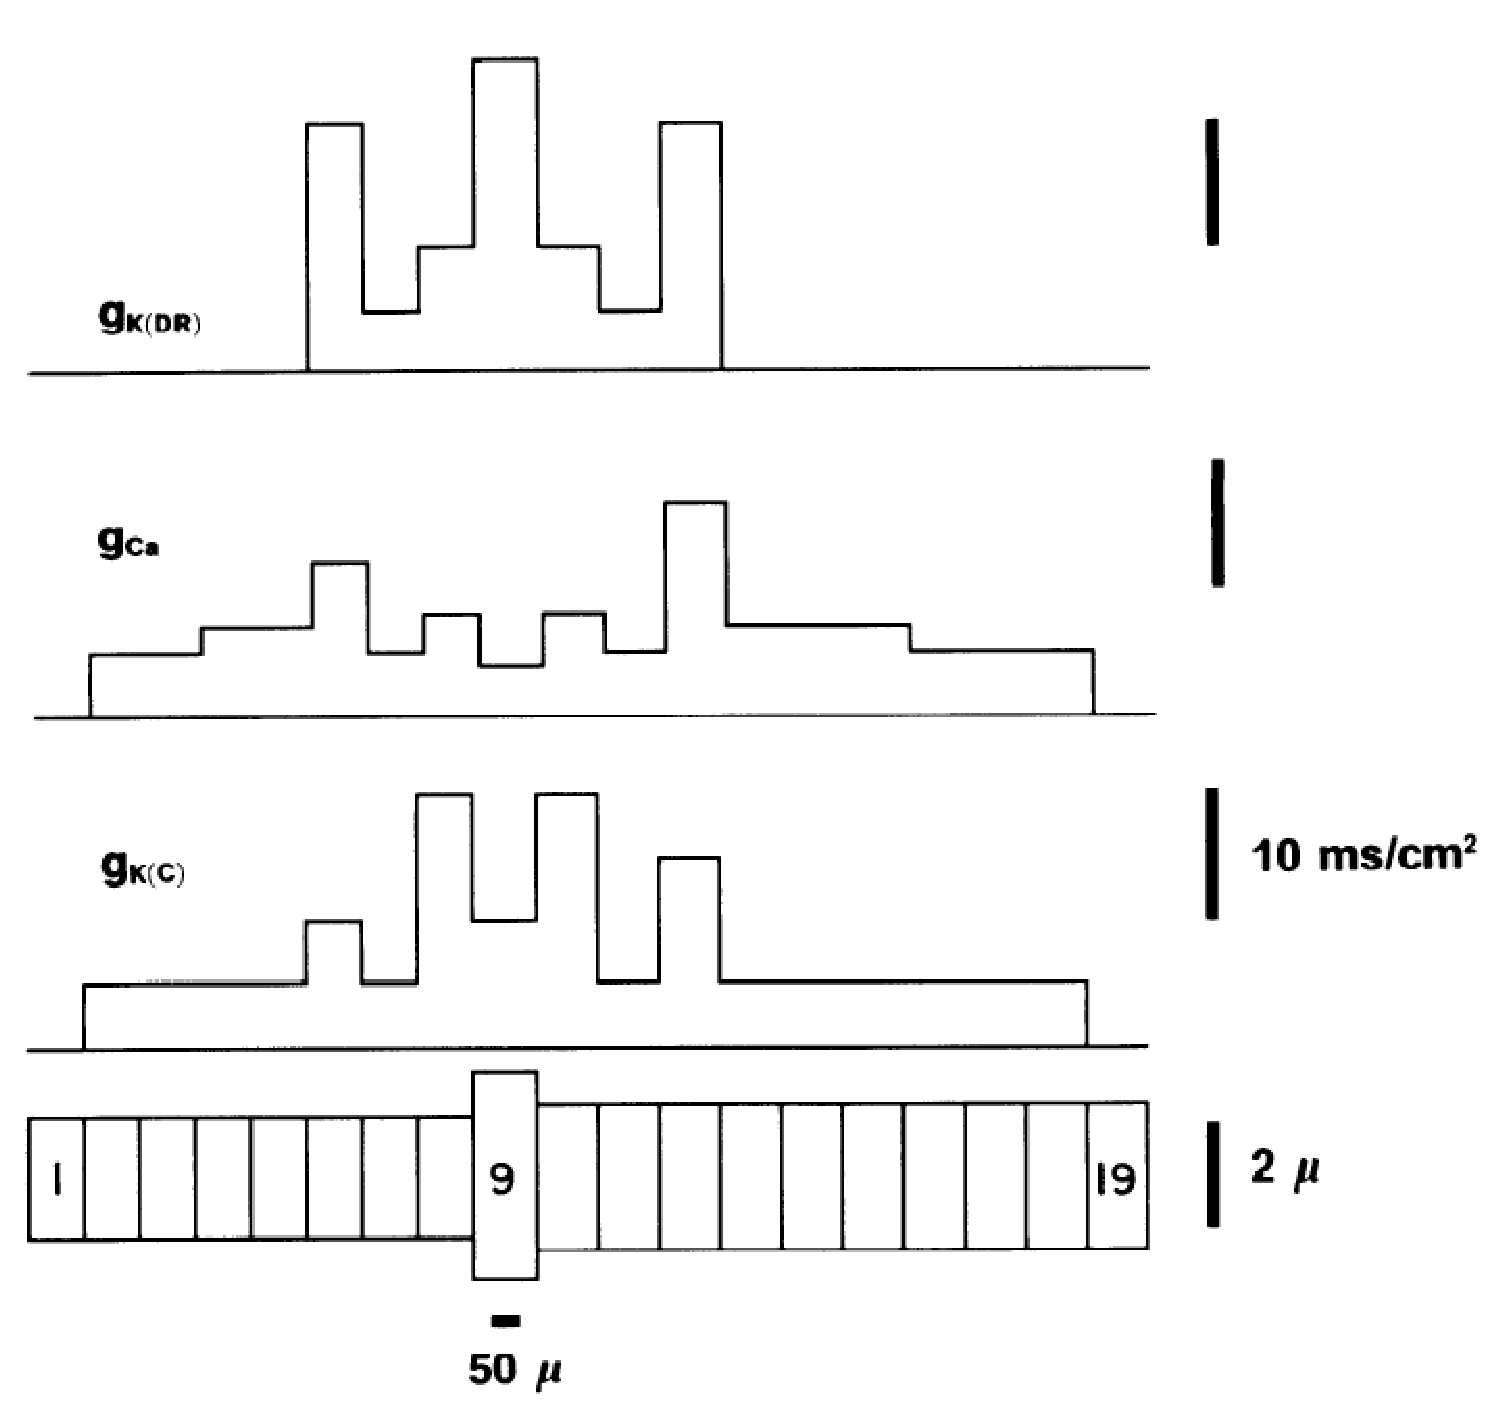
\includegraphics[height=5.5cm,
    angle=0]{./images/traub_ion_distribution_CA1.eps}}
\centerline{(A)j \;\;\;\;\;\;\;\;\;(B)}
  \caption{Distribution of 4 of the ionic currents on each compartment
    - compartment 9 is the soma, compartments on the left is for
    basilar dendrites, on the right is for apical dendrites. Note the
    scale on horizontal and vertical are different. Conductance
    density is drawn over each compartment according to the scale on
    the right (10mS/cm$^2$): (A) CA3 cell, (B) CA1 cell with
    $g_{\ce{Na}}$ the same as that in CA3 cell}
\label{fig:traub_ion_distribution}
\end{figure}



\subsection{Assumptions}
\label{sec:assumptions-2}

Assumptions:
\begin{enumerate}
\item Extracellular space is isopotential

\item The distribution of membrane conductances densities as given in
  Fig.~\ref{fig:traub_ion_distribution}, with $g_{\ce{K(A)}}$ only in
  soma. 

\item The leakage current is constant, i.e. independent of the
  membrane potential
\item The model doesn't use the whole cell intracellular \ce{Ca^2+}
  concentration, yet at a submembrane ``virtual shell'' $\chi$. This
  restriction is due to computationally intensive%  as it requires to
  % take into account the mechanism to release calcium from internal
  % storage)

\item The ionic behavior is derived from Hodgkin-Huxley model

\item The inverse time constant for (1st-order) relaxation of $\chi_k$
  are assumed to be the same for all compartments, and is equal to
  $0.075$ms$^{-1}$, corresponding to a time constant of
  13.33ms$^{-1}$.
\item Calcium current is converted to \ce{Ca^2+} concentration via
  scaling factors $\phi_k$ 
\item The synaptic current is excitatory only and occur on two
  compartments: number 3 and 15, each $0.6\lambda$ from the soma (one
  on the basilar, one on the apical dendrite). 
\item The model can be applied to both CA1 and CA3 cell; they differ
  only in the conductances' values.
\end{enumerate}

Traub's 19-compartment model~\citep{traub1991ca3} has the following
property and characteristic.

\begin{itemize}
\item each compartment has 6 ionic currents whose kinetics were
  constructed using {\it somatic-clamp data} from different
  researchers' works.
\item steady somatic injected current ($I_s$):
  \begin{itemize}
  \item weak $I_s$: low frequency (1Hz) bursting; higher $I_s$: higher
    frequency, up to 8Hz
  \item intermediate $I_s$: aperiodic behavior
  \item high $I_s$: periodic spiking
  \end{itemize}
\item steady dendritic injected current ($I_d$):
  \begin{itemize}
  \item a larger range of bursting frequencies (1-20Hz)
  \end{itemize}
\end{itemize}

\subsection{Conventions}
\label{sec:conventions}

Conventions:
\begin{enumerate}
\item Units: mV, nA, ms, nF,and $\mu$S.
\item The second subscript (denoted by $k$) is used to index the
  compartment ($k=1..19$)
\item Membrane potential is written relative to resting potential
  $V_k=V_{m,k}-E_{r,k}$ ($k=1..19$)
\item Letter C is used for capacitance, $C_k$
\item Subscript L is used for leak conductance or current
\item Na, K, Ca refer to respective ions
\item $V_{\ce{Na}}, V_{\ce{K}}, V_{\ce{Ca}}$ are constants (equilibrium
  potentials) 
\item The bar superscript, as in $\overline{g}_{\ce{Na}}$, denotes maximum
  ionic conductance of a particular type in a particular compartment
\item There are 4 types of potassium currents: K(DR), K(A), K(AHP),
  K(C)
  \begin{itemize}
  \item DR = delayed rectifier
  \item A = A-type of transient current
  \item AHP = after hyperpolarization (long-duration Ca-dependent AHP
    current) 
  \item C = short-duration Ca- and voltage-dependent current
  \end{itemize}
\item Dimensionless membrane-state variables that control the various
  ionic conductances are $m,h,s,r,n,a,b,q$ and $c$ (in the range
  0..1).
\item Calcium concentration in a ``shell'' beneath the membrane
  compartment is $\chi$. This local ``virtual shell'' concentration
  increases by transmembrane influx of Ca (intracellular release are
  not being considered) and declines by first-order decay with time
  constant $\beta_\chi^{-1}$. $\chi$ regulates the local AHP and C
  conductances.
\end{enumerate}

\subsection{Procedures}
\label{sec:procedures}


What they did in simulation?
\begin{enumerate}
\item Inject a current at different place (soma, $0.3\lambda$,
  and $0.6\lambda$ of the apical dendrite)
\item Simulation on a network with 100 or 1000 cells.
\end{enumerate}

What we expect the model to reproduce?
\begin{enumerate}
\item a burst in one CA3 cell can initiate a burst in the postsynaptic
  pyramidal cell
\item a single cell can synchronize the entire population
  (synchronized population oscillations)
\end{enumerate}

\subsection{Mathematical model}
\label{sec:mathematical-model-3}

The model has
\begin{itemize}
\item 288 parameters (constants)
\item 189 variables
\item ... equations
\end{itemize}

The currents in a compartment involves: axial current in from the
previous compartment (if not soma) and axial current out to the next
compartment (if not the final compartment) and ionic current.
\begin{eqnarray}
  \label{eq:534}
  C_k\frac{dV_k}{dt} = \gamma_{k-1,k} (V_{k-1}-V_k) +
  \gamma_{k+1,k}(V_{k+1}-V_k) - I_{ionic,k}
\end{eqnarray}

The ionic current is composed of leak current, synaptic current, 6
ionic currents, and injected current (if available).

\begin{equation}
  \label{eq:535}
  \begin{split}
  I_{k} = &g_{L,k}V_k + I_{synaptic,k} +
  \overline{g_{\ce{Na}}}m_k^2h_k(V_k-V_{\ce{Na}}) +
  \overline{g_{\ce{Ca}}}s_k^2r_k(V_k-V_{\ce{Ca}}) +\\
  &\overline{g_{\ce{K(DR)}}}n(V_k-V_{\ce{K}}) +
  \overline{g_{\ce{K(A)}}}ab(V_k-V_{\ce{K}}) +
  \overline{g_{\ce{K(AHP)}}}q(V_k-V_{\ce{K}}) + \\
  &\overline{g_{\ce{K(C)}}}\times c
  \times \min\left(1,\frac{\chi_k}{250}\right)\times (V_k-V_{\ce{K}}) -
  I_{injected,k}
  \end{split}
\end{equation}

Using steady-state values of the electrotonic parameters, as shown in
Table~\ref{tab:steady-state_traub}~\citep{turner1980sse}:
\begin{table}[hbt]
\begin{center}
\caption{Steady-state values}
\begin{tabular}{cc} 
  \hline
  parameters & parameters \\ 
  \hline\hline
  $R_i=100\Omega$cm & \\
  $R_m=10,000\Omega$cm$^2$ & \\
  $C_m=3\mu$F.cm$^{-2}$ & \\
  $\tau_M=30$ms & \\
  $R_{ad}=60M\Omega$ & input resistance apical dendrite\\
  $R_{bd}=90M\Omega$ & input resistance basilar dendrite\\
  $R_{wc}=32M\Omega$ & input resistance whole cell\\
  radius 4.23$\mu$m, length 125$\mu$m,  & soma
  dimension\\
  area 3,320$\mu$m$^2$  & (shape is not realistic, yet area is
  reasonable) \\
  radius 2.89$\mu$m, length 120$\mu$m,  & apical compartment
  \\  
  area 2.188$\mu$cm$^2$  & \\
  radius 2.42$\mu$m, length 110$\mu$m,  & basilar compartment
  \\  
  area 1,673$\mu$cm$^2$  & \\  
\end{tabular}
\end{center}
\label{tab:steady-state_traub}
\end{table}

Based on apical compartment data, $1\lambda$ = 1,2000$\mu$m=1.2cm),
this is consistent with the result 
\begin{eqnarray*}
  \lambda = \sqrt{\frac{rR_m}{2R_i}} =
  \sqrt{0.00289\times10,000/(2\times 100)} = 0.120 \text{cm}
\end{eqnarray*}


\subsection{Numerical analysis}
\label{sec:numerical-analysis}

They used 2nd-order Taylor series method, with a fixed time step of
50$\mu$s. Data was outputted every 0.25ms of a simulation. 

\subsection{Summary}
\label{sec:summary-1}

\begin{enumerate}
\item There are different types of firing behavior, elicited by (1)
  brief current pulse, (2) small, (3) large depolarizing current
  injected into the soma.
\item There are still low-amplitude oscillation, in which there are
  both regular rhythm, as well as irregular pattern of firing. 

\end{enumerate}

\section{Traub et al. (1993) - CA3 region network}


A model of the isolated CA3 region, in vitro very much along the lines of Traub,
Mliles \& Buzsaki (1992).
\begin{itemize}

  \item   (using 100 pyramidal neurons in 10x10 array, with 20 or 50
  interneurons).
  
  \item half of interneurons generate GABA-A IPSP; and half of interneurons
  generate GABA-B ISPSP

  \item Pyramidal neurons are designed to have sufficiently many inputs from
  interneurons, e.g. at least 20 GABA-A inputs (Miles and Wong, 1987)
  
  Here, each pyramidal neuron has inputs from 20 other pyramidal neurons; and
  from 12-40 inhibitory interneurons.
  
  Each inhibitory interneuron has input from 20 pyramidal neurons.
  
  \item synaptic connections are constructed randomly 
\end{itemize}
Statistics were collected from 160 simulations; each at least 750ms of neuronal
behavior.

The single neuron model is based on Traub et al. (1991) - Sect.\ref{sec:Traub-1991}



\section{Traub et al. (1994) - CA3 pyramidal cell}
\label{sec:Traub-1994-pyramidal}

An improvement of previous model (Sect.\ref{sec:Traub-1991})
\begin{enumerate}
  \item branched dendrite:
 
Still impose artificial symmetry on the branches to reduce the number of
parameters


  \item added axon and IS: with higher $g_\na$ than that in soma, besides
  different Na+ channel kinetics.
  
  \item 
\end{enumerate}

\section{Traub et al. (1995) - interneuron}
\label{sec:Traub-1995-interneuron}

\begin{enumerate}
  \item 51 compartments: 46 soma-dendritic (SD)D compartments + 1 IS compartment
  + 4 axonal compartments
  
  \item 
\end{enumerate}
Each compartment is characterized by length (l), radius (r) and surface area
(A): A = $2\pi .r. l$ (no spines taken into account).

The model for interneuron is derived based upon that for pyramidal neuron -
Sect.\ref{sec:Traub-1994-pyramidal}, with changes
\begin{enumerate}	
  \item much higher gNa, gK(DR)
  
  \item lower gCa, gK(C)
  
  \item E(rev)-K is -25mV relative to rest
  
  \item more rapidly decay somatic Ca2+
\end{enumerate}



\section{Pinsky-Rinzel (1994) - CA3 pyramidal cell}
\label{sec:Pinksy-Rinzel-1994}


\subsection{Motivation}
\label{sec:motivation-1}

Should we create a minimal biophysical/mathematical model that can reproduce
Traub's result (Sect.\ref{sec:Traub-1991})? 

Pinsky and Rinzel has developed a two-compartment with 8 variable model of CA3
pyramidal cell. They reduce the number of compartments, yet the ionic currents
and gating in a single compartment are retained~\citep{pinsky1994inr}.
\begin{itemize}
\item two compartments: soma and dendrite
\item coupling conductance between the two compartments is $g_c$
  (electrotonic parameter):
  \textcolor{red}{bursting can occur only with a limited range of
    $(g_c,p)$ only, e.g. either extreme small $g_c$ (decoupled
    compartment) or large $g_c$ (isopotential cell, i.e. no difference
    between the two compartment)}
\end{itemize}

With two dendrites, one for sensoring and one for firing signals, a
pyramidal neurons receive multiple inputs. The incoming electrical
signal can be from different class of stimulus. In other words, each
input is for a particular class of job, where all jobs within one
class have a fixed route through the network.

Under the assumption that there are several classes of jobs, the input
stream to each neuron is the superposition of several individual
streams yielding a net stream with {\bf Poisson characteristics}. It
has also been proved that when many independent incoming processes are
added together, the resultant arrival process tends to be Poisson even
if the individual processes are not [Richard M. Fieldman, Ciriaco
Valdez-Flores, Applied Probability and Stochastic Processes, 8.2.1].
\textcolor{red}{So, Poisson input streams arises in systems with a
  large number of feedback loops}.

Idea: Jackson network (section 8.1. of Applied Prob. and Stochastic
Proc.]

\begin{figure}[hbt]
  \centerline{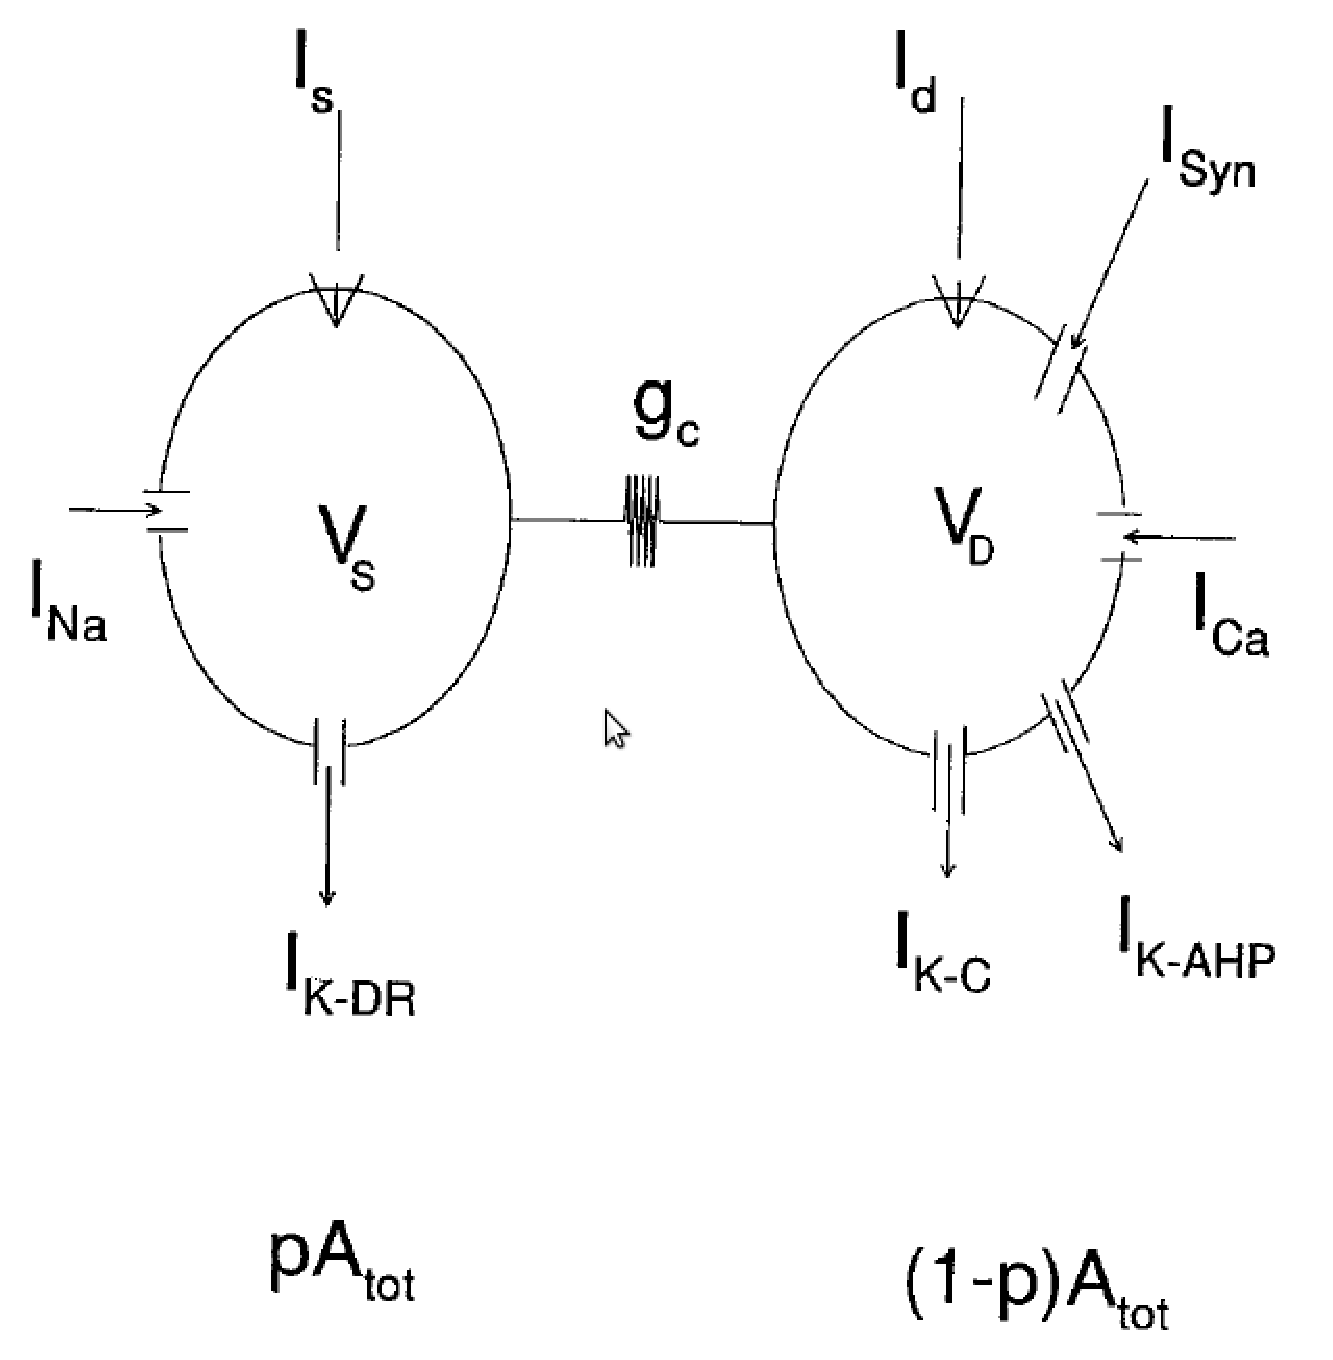
\includegraphics[height=5cm,
    angle=0]{./images/pinsky-rinzel.eps}}
  \caption{Schematic diagram of two-compartment model($A_{tot}$ is the
    total cell membrane area which is normalized to 1)}
  \label{fig:pinsky-rinzel}
\end{figure}

\subsection{Formulation}
\label{sec:formulation-1}

Ionic currents in each compartment:
\begin{itemize}
\item soma: two spike-generating currents, they are inward sodium
  $I_{\ce{Na}}$, and outward delay-rectifier $I_\Kdr$, as well as the
  leak $I_{L,1}$.
\item dendritic: high-threshold inward calcium $I_{Ca}$
  (voltage-dependent), and two types of potassium currents $I_{K-C}$
  (voltage-dependent $Ca$-activated), $I_{K-AHP}$ (voltage-independent
  calcium-activated), as well as the leak current $I_{L,2}$.
\end{itemize}
The current balance equations for the two compartments:
\begin{equation}
  \label{eq:563}
  \begin{split}
    C_m\frac{dV_s}{dt} &= -I_{L,1} - I_{Na} - I_\Kdr  -
    \frac{g_C}{p}.(V_s-V_d) + I_{s}/p \\
    C_m\frac{dV_d}{dt} &= -I_{L,2} - I_{Ca} - I_{K-AHP} - I_{K-C} -
    \frac{g_C}{(1-p)}.(V_d-V_s) - I_{syn}/(1-p) + 
I_d/(1-p)
  \end{split}
\end{equation}
with current unit is $\mu$A/cm$^2$; and
\begin{itemize}
\item capacitance $C_m$ ($\mu$F/cm$^2$)
  \begin{eqnarray*}
    C_m = 3\mu F/cm^2
  \end{eqnarray*}
\item time (ms)
\item $V_s,V_d$ (mV) are the deviation of the somatic, and dendritic
  membrane potential from the reference potential of $-60$ mV. 
  \begin{eqnarray*}
    V_s = V_{m,s}-(-60) \\
    V_d = V_{m,d}-(-60)
  \end{eqnarray*}
\item conductance $g_c, \overline{g_L},\overline{g_{Na}},
  \overline{g_K},\overline{g_{Ca}}$ (mS/cm$^2$)

  the coupling conductance $g_c= 2.1$ which is different from the
  value computed from axial resistance $R_i,r$ and $l$,
  i.e. $g_c\approx 0.18$. The reason is that this value is too small
  to generate spike. The detect of the value $g_c=2.1$ was chosen so
  that it maximize  TAF (transient attenuation factor) at dendrite
  \begin{eqnarray*}
    TAF = \frac{V_{d,max}-V_{d,ss}}{V_{clamp}-V_{hold}}
  \end{eqnarray*}

\item $I_{L,1}(V_s), I_{L,2}(V_d)$ ($\mu$A/cm$^2$): 
  \begin{eqnarray*}
    I_{L,1} &&= \overline{g_L}(V_s-V_L) \\
    I_{L,2} &&= \overline{g_L}(V_d-V_L) \\
    \overline{g_L} &&= 0.1
  \end{eqnarray*}

\item $I_{Na}(V_s,h)$: the Hodgkin-Huxley model of Na channel is used.
  \begin{eqnarray*}
    I_{Na} &&=\overline{g_{Na}}m_\infty^3(V_s).h.(V_s-E_{Na}) \\
    \overline{g_{Na}} &&= 30 \\
    E_{Na} &&= 120 \\
    \frac{dh}{dt} &&= \frac{h_\infty-h}{\tau_h}\\
    h_\infty &&= \frac{\alpha_h}{\alpha_h+\beta_h} \\
    \tau_h &&=  \frac{1}{\alpha_h+\beta_h} \\
    \alpha_h &&= 0.128\exp(\frac{17-V_s}{18})\\
    \beta_h &&= \frac{4}{1+\exp(\frac{40-V_s}{5})}
  \end{eqnarray*}
due to the instantaneous activate of Na current, the activating gating
variable $m$ is approximated by its steady-state value
$m_\infty(V_s)$. 
\begin{eqnarray*}
  m_\infty = \frac{\alpha_m}{\alpha_m+\beta_m}\\
\alpha_m = \frac{0.32(13.1-V_s)}{\exp(\frac{13.1-V_s}{4}-1)}\\
\beta_m = \frac{0.28(V_s-40.1)}{\exp(\frac{V_s-40.1}{5}-1)}
\end{eqnarray*}

\item $I_{Ca}(V_d,s)$: use Ca kinetics from pyramidal neuron in CA1
  region~\citep{kay1987cca}.
  \begin{eqnarray*}
    I_{Ca} = \overline{g_{Ca}}.s^2.(V_d-E_{Ca}) \\
    \overline{g_{Ca}} = 10 \\
    E_{Ca} = 140 \\
\frac{ds}{dt} = \frac{s_\infty-s}{\tau_s} \\
s_\infty = \frac{\alpha_s}{\alpha_s+\beta_s} \\
\tau_s =  \frac{1}{\alpha_s+\beta_s} \\ 
\alpha_s = \frac{1.6}{1+\exp(-0.072(V_d-65))} \\
\beta_s = \frac{.02(V_d-51.1)}{\exp(\frac{V_d-51.1}{5})-1}
  \end{eqnarray*}
\item $I_{K-C}(V_d,Ca,c)$ is proportional to fast activation variable
  $c$ times a saturating function $\chi(Ca)$, with $Ca$ is
  intracellular free calcium level in a sub-membrane ``shell'' of the
  dendritic compartment. $Ca$ is unitless.
  \begin{eqnarray*}
    I_{K-C} = \overline{g_{K-C}}. c.\chi(Ca).(V_d-E_K)\\
    \overline{g_{K-C}} = 15\\
    E_{K} = -15 \\
    \frac{dc}{dt} = \frac{c_\infty-s}{\tau_c} \\
    c_\infty = \frac{\alpha_c}{\alpha_c+\beta_c} \\
    \tau_c =  \frac{1}{\alpha_c+\beta_c} \\ 
   \left\{
       \begin{array}{lc}
         \alpha_c =
         \frac{\exp(\frac{V_d-10}{11})-\exp(\frac{V_d-6.5}{27})}{18.975}&\;\;
         \text{for } V_d\le 50 \\
         \alpha_c = 2.\exp(\frac{6.5-V_d}{27})& \;\; \text{for } V_d > 50 
       \end{array}\right.\\
     \left\{
         \begin{array}{lc}
           \beta_c = 2.\exp(\frac{6.5-V_d}{27}) - \alpha_C
           &\;\;
           \text{for } V_d\le 50 \\
           \beta_c = 0& \;\; \text{for } V_d > 50 
         \end{array}\right. \\
       \chi(Ca) = min(Ca/250,1)
  \end{eqnarray*}

\item $I_{K}$ here is the delayed rectifier $I_\Kdr(V_s,n)$
  \begin{eqnarray*}
    I_\Kdr &&= \overline{g_\Kdr}.n.(V_s-E_K) \\
    \overline{g_\Kdr} &&= 15\\
    \frac{dn}{dt} &&= \frac{n_\infty-n}{\tau_n}\\
    n_\infty &&= \frac{\alpha_n}{\alpha_n+\beta_n} \\
    \tau_n &&=  \frac{1}{\alpha_n+\beta_n} \\
    \alpha_n &&= \frac{0.016(35.1-V_s)}{\exp(\frac{35.1-V_s}{5}) - 1} \\
    \beta_n &&= 0.25\exp(.5-.025V_s)
  \end{eqnarray*}

\item $I_{AHP}$ is the slow AHP Ca-activated \ce{K+} channel
  $I_{K-AHP}(Ca,q)$.
  \begin{eqnarray*}
    I_{K-AHP} = \overline{g_{K-AHP}}. q .(V_d-E_K) \\
    \overline{g_{K-AHP}} = 0.8 \\
    \frac{dq}{dt} =  \frac{q_\infty-s}{\tau_q} \\
    q_\infty = \frac{\alpha_q}{\alpha_q+\beta_q} \\
    \tau_q =  \frac{1}{\alpha_q+\beta_q} \\ 
    \alpha_q = \min((0.00002)Ca,0.01)\\
    \beta_q = 0.001
  \end{eqnarray*}
\item $I_{s},I_{d}$ is the electrode current applied to the soma
  and dendrite
  \begin{eqnarray*}
    I_s = -0.5 \\
    I_d = 0.0
  \end{eqnarray*}
\item $p$ is the area ratio between the soma and the whole cell 
  \begin{eqnarray*}
    p = \frac{\text{area soma}}{\text{area soma + area dendrite}}
  \end{eqnarray*}
we choose $p=0.5$. 
\end{itemize}

Another assumption is that $Ca$ does not diffuse between compartment,
so the equation for \ce{Ca^2+} handling in the dendritic compartment
is
\begin{eqnarray}
  \label{eq:564}
  \frac{dCa}{dt}= -0.13 I_{Ca} - 0.075 Ca
\end{eqnarray}
All gating variable $h,s,c,q,n$ follow the first-order kinetics
\begin{eqnarray}
  \label{eq:565}
  y' = \frac{y_\infty(U)-y)}{\tau_y(U)}
\end{eqnarray}
with $U=V_s$ when $y=h,n$, $U=V_d$ when $y=s,c$; and $U=Ca$ when
$y=q$.


\subsection{Parameter settings}
\label{sec:parameter-settings}

Initial values for the simulation are chosen from stable rest state.
\begin{eqnarray*}
  V_s &&= -4.6 mV \\
  V_d &&= -4.5 mV \\
  h &&= 0.9999 \\
  n  &&= 0.001 \\
  s &&= 0.009 \\
  c &&= 0.007 \\
  q &&= 0.010 \\
  Ca &&= 0.2 
\end{eqnarray*}

$I_s=-0.175\mu$A/cm$^2$ (p=0.5). The isolated soma show a wide range
of frequencies for $I_s$ of low to max rate around 300 Hz.


\section{Wang (1998) - spike-frequency adaptation)}
\label{sec:wang-model}

\subsection{Motivation}
\label{sec:motivation}


The outstanding behavior of cortical neurons is that in response to a
constant current pulse (at various time length) at the dendrite (or
postsynaptic cell), the (soma of the) cell may produce different
firing patterns (read Sect.~\ref{sec:volt-activ-ionic}).  Under a
stimulus (square injected current pulses), the adaptation time course
of cortical cells can be fitted empirically by an exponential time
course
\begin{equation}
  \label{eq:339}
  f(t) = f_{ss} + (f_0-f_{ss}) \exp(-t/\tau_{adap})
\end{equation}
with $f_0$ is initial firing rate, $f_{ss}$ is steady-state firing
rate and $\tau_{adap}$ is {\it adaptive (membrane) time constant}. This time
course is characterized by two quantities
\begin{itemize}
\item $\tau_{adap}$
\item $F_{adap} = \frac{f_0-f_{ss}}{f_0}$. 
\end{itemize}
which vary widely between superficial and deep layer neurons,
i.e. $\tau_{adap}=10-50$msec. and $F_{adap}=50-70$\%.

In this study, the author \citep{wang1998cca} aimed to solve $\tau_{adap}$ and
$F_{adap}$ analytically based on cellular physiological parameters, rather based
on empirical parameters. In other words, \textcolor{blue}{this is the
quantitative study of spike-frequency
  adaptation temporal dynamics}.
\textcolor{red}{This spike-frequency adaptation is assumed to depend on
voltage-independent, \ce{Ca^2+}-gated \ce{K+} currents ($I_{AHP}$);} although
other types of \ce{K+} currents (e.g. ``M'' currents) also involves in a lesser
degree. The intrinsic gating of $I_{AHP}$ is rapid; thus its slow activation is
attributed to the kinetics of the cytoplasmic $[\ce{Ca^2+}]_i$. The dynamics of
$[\ce{Ca^2+}]_i$ can be measured accurately in pyramidal
neuron~\citep{helmchen1996cba}.

\subsection{Background}
\label{sec:background}

This paper (\citep{wang1998cca}) uses Pinsky and Rinzel model
(sect.~\ref{sec:Pinksy-Rinzel-1994}) with 2 compartments:
\begin{itemize}
\item dendrite
\item soma plus axonal initial segment.
\end{itemize}
The reason of using 2-compartment model is that 
\begin{enumerate}
\item the [\ce{Ca^2+}] in dendrite are much larger than in the soma,
  the change in calcium concentration are primarily by \ce{Ca^2+}
  entry at voltage-gated \ce{Ca^2+} ion channels in the dendrites.
  \textcolor{red}{This model focuses on spike-frequency adaptation
    that is caused by dendritic [\ce{Ca^2+}]-dependent $I_{AHP}$}.
\item They want to test the hypothesis: if there are two or more
  calcium modes, i.e. another $I_{AHP}$ in the soma, then the
  spike-frequency adaptation should be the sum of two exponentials.

\item The cell can display a burst firing patterns, requiring only a
  weak electrotonic interaction $g_c$ between the two compartments.
\end{enumerate}

\subsection{Formulation}
\label{sec:formulation}

The cell can be excited by either
\begin{itemize}
\item an injected current $I_{s}$ ($\mu$A/cm$^2$) at the soma
\item (normally distributed) random synaptic input $I_{syn}$ to the
  dendrite (with
  $\alpha$-amino-3-hydroxy-5-methyl-4-isoxazolepropionic acid type).
  \begin{eqnarray}
    \label{eq:553}
    I_{syn} = g_{syn}.s.(V-E_{syn})
  \end{eqnarray}
  with $s$ is the gating variable obeying the equation 
  \begin{eqnarray}
    \label{eq:554}
    \frac{ds}{dt}= \eta(t) - \frac{s}{\tau_s}
  \end{eqnarray}
  with $\eta(t)$ is a Poisson-point process with rate $\lambda$ (can be
  chosen different values to test, e.g. $\lambda = 0.3, 1.0, 1.5,$ or
  $2.5$ kHz). $E_{syn} = 0$mV, $\tau_s=0.5$ms, $g_{syn}=0.08$mS/cm$^2$
  (if present). 
\end{itemize}

Besides, there are ionic currents in each compartment:
\begin{enumerate}
\item in the soma: leak current, $I_{L,s}$, a spike generating
  currents $I_{\ce{Na}}$ and $I_{\ce{K}}$, and
  \textcolor{red}{possibly $I_{\ce{Ca}}$ and $I_{AHP(s)}$}\footnote{red
    color = new compared to Pinsky-Rinzel model}, as well as
    the current from the dendrite.

  \item in the dendrite: the leak current $I_{L,d}$, high-threshold
    calcium current (via L-type channels) $I_{Ca}$ and
    calcium-activated \ce{K+} current $I_{AHP(d)}$, as well as the current
    from the soma\footnote{$I_{K-C}$ in Pinsky-Rinzel is not used}.
\end{enumerate}
NOTE: We use $I_{AHP(s)}$ and $I_{AHP(d)}$ to differentiate the slow
AHP \ce{K+} currents at two different compartments. However, the paper
assumed they are the same. 

Then, using Ohm's law, the somatic $V_s$ and dendritic $V_d$ membrane
potential follow the current-balance equation.
\begin{eqnarray}
  \label{eq:340}
  C_m\frac{dV_s}{dt} &= -I_{L,s} - I_{Na} - I_K - I_{Ca} - I_{AHP(s)} -
  \frac{g_C}{p}.(V_s-V_d) + I_{s} \\
  C_m\frac{dV_d}{dt} &= -I_{L,d} - I_{Ca} - I_{AHP(d)} -
  \frac{g_C}{(1-p)}.(V_d-V_s) - I_{syn} 
\end{eqnarray}
with (the same for both soma and dendrite) $C_m = 1\mu$F/cm$^2$ , the
leak current $I_{L,i}=g_L(V_i-V_L)$ with $i=s,d$. The weak coupling
conductance between the soma and the dendrite is $g_C$. So, the
current between the soma and the dendrite (in $\mu$A/cm$^2$) is
assumed to proportional to $(V_s-V_d)$ with the coupling conductance
$g_c=2$mS/cm$^2$, and the area ratio
$p=\frac{\text{somatic
    area}}{\text{total area}}=0.5$~\citep{pinsky1994inr}.


All voltage-dependent currents are described by Hodgkin-Huxley
formalism (sect.~\ref{sec:Hodgkin-Huxley-1952-model}) with the temperature
factor $\Phi = 4$. The dynamics of the gating variables are
\begin{equation}
  \label{eq:561}
  \frac{dx}{dt} = \Phi_x.\left[ x_\infty(V) - x\right]/\tau_x(V)
\end{equation}
with $x = n, h$; except for the fast activating variable $m$ of the
sodium current which is approximated by the steady-state $m_\infty$.
\begin{eqnarray}
  \label{eq:556}
I_{K} &= \overline{g_K} .n^4.(V_m-E_K) \\
  I_{Na} &= \overline{g_{Na}} .m^3_\infty(V_m).h.(V_m-E_{Na})
\end{eqnarray}
with $m_\infty=\frac{\alpha_m}{\alpha_m+\beta_m}$, 
\begin{eqnarray}
  \label{eq:557}
  \alpha_m &= \frac{0.1(V_m+33)}{1-\exp(-0.1(V_m+33))}\\
\beta_m &=  4\exp\left[-(V_m+58)/12\right] \\
h(\cdot) = h_\infty  - (h_\infty - h0)
\end{eqnarray}

{\bf NOTE}: The constant values used in those formulas are different
from those used by Hodgkin-Huxley model.


The high-

Input:(all in double precision)
\begin{verbatim}
Vm     =         ! Vm = V  (membrane voltage)
Vs     =         !mV
Vd     =         !mV
Cm     = 1       !uF/cm^2  (capacitance)
   ! conductances
gc     =  2      !mS/cm^2  (coupling conductance)
gL     =         !mS/cm^2
g_syn  = 0.08    !mS/cm^2
gNa_bar =

I_s    =         ! injected applied current to the soma
p      = 0.5d0   ! somatic area/total area
E_syn  = 0       !mV
tau_s  = 0.5     !ms
lambda = 0.3d0   !kHz, other choices: 1.0d0, 1.5d0, 2.5d0

! initial values
s =              ! gating variable
dt = 
! initialize seed RNG (poisson)
 ....
! initialize seed RNG (normal)

!begin integration loop
  ! generate normal random number rn_norm
  
  I_syn = g_syn*s*(Vm-E_syn)    ! random synaptic input

  !ds/dt = eta(t) - s/tau_s  (Euler)
  eta = poissonpoint(lambda)  
  s = s + dt*(eta - s/tau_s)

  ! dVs/dt (Euler)
  Vs = Vs + dt*(-I_L-I_Na-I_K-I_AHPs - gc*(Vs-Vd)/p+I)/(Cm)
  ! dVd/dt (Euler)
  Vd = Vd + dt*(-I_L-I_Ca-I_AHPd - gc*(Vd-Vs)/(1-p)+I_syn)/(Cm)
     ! adapt time-step dt ???
  I_L    = gL *(Vm - E_L)               ! leak current (uA)
  I_Na   = gNa_bar*(m_inf**3)*h* (Vm-E_Na)   ! sodium current (uA)
  I_K    = gK_bar**(n**4) * (Vm-E_K)        !uA
  I_Ca   =         !uA
  I_AHPs =         !uA
  I_AHPd = I_AHPs  !uA

h_0 = ...
alpha_m = 0.1d0*(Vm + 33d0)/(1-exp(-0.1d0*(Vm+33d0)))
beta_m = 4d0*exp(-(Vm+58d0)/12d0)
m_inf = alpha_m/(alpha_m + beta_m)
!dh/dt
h = Phi*(h_inf - (h_inf - h_0) * exp(-time/tau_h))
h_inf = alpha_h/(alpha_h + beta_h)
tau_h = 1/(alpha_h+beta_h)
alpha_h = 0.07d0*exp(-(Vm+50d0)/10d0)
beta_h = 1/(exp(-0.1d0*(Vm+20d0))+1)
n = Phi
 
!end integration loop
\end{verbatim}


References:
\begin{itemize}
\item \url{http://www.neuron.yale.edu/phpBB/viewtopic.php?f=8&t=416}:
  Random synaptic input 
\end{itemize}


\section{Hoffman et al. (1997) - CA1 pyramidal neurons}
\label{sec:Hoffman-1997-pyramidal-CA1}

\citep{hoffman1997} showed that dendrites of CA1 pyramidal neurons  have a high
density of transient A-type $\K$ channels and the density increases wit distance
from soma (Sect.\ref{sec:A-type-K+current}).

The presence of the strong outward current causes action-potential amplitude to
decrease with distance from the soma, inhibits the ability of dendrites to
initiate action potentials, and alters the shape of EPSPs.
A-type K+ channels play the dominant role in determining the electrical
properties of CA1 dendrites and thereby influence dendritic integration and
propagation of information.

\subsection{Parameters}

$R_m = 30,000 \Omega.\cm^2$ and $\Csc = 1\muF/cm^2$ (somatic compartment) and
$\Csc = 1.6\muF/\cm^2$ (dendritic compartments to account for spines).
Axial resistivity $R_a = 150 \Omega.\cm$, ecept in axon $R_a = 100 \Omega.\cm$.

\subsection{Model synaptic input}
\label{sec:EPSP-model-synaptic-input-Hoffman1997}

Synaptic input is modeled as an injected current with a conductance with dual
exponential time course of form: $g_\syn = (1-e^{-t/\tau_1})(e^{-t/\tau_2})$.
with $t=0$ is the onset of the conductance ($\tau_1 = 1.5$(ms), and 
$\tau_2 = 5-10$(ms)).
\begin{equation}
I_\syn = g_\syn (V_m - E_{\rev,\syn})
\end{equation}
Reversal potential of synapse $E_{\rev,\syn}=0$(mV).

EPSPs of 15-20mV (Sect.\ref{sec:EPSP}) near the site of input were produced by
5-7 simultaneously activated synaptic conductances distributed along $\approx
50\mum$ of dendrite.


\subsection{Numerical method}

Model was built using NEURON (Sect.\ref{sec:NEURON}) with $\Delta t = 0.025$
(ms).


\section{Colbert - Pan (2002)}
\label{sec:Colbert-Pan-2002}

They made computer simulations using NEURON software. The model was
similar to that described in Hoffman et al.
(Sect.\ref{sec:Hoffman-1997-pyramidal-CA1}) with some modifications.
Simulations assumed a temperature of 23$^\circ$C.

$\Na$ channels are different in AIS vs. other regions
\begin{itemize}
  \item 3x higher in conductance
  \item $V_{1/2}$ is -38mV in AIS, while in initial segments and other regions:
  -31mV
\end{itemize}

\section{Schaefer (xxxx)}

The model is capable of replicating the BAC firing; however it does not produce
the typical f-I curve and perisomatic step current firing behavior of these
cells.

\section{Kole (xxxx)}

The model fits the shape of a single spike at the
axon, soma and dendrites, but is incapable of generating apical
Ca2+ spikes and does not capture the f-I curve or perisomatic step
current firing.

%%% Local Variables: 
%%% mode: latex
%%% TeX-master: "mainfile"
%%% End: 
\section{Hay et al. (2011) = Layer V5 cortical pyramidal cell}
\label{sec:Hay-2011}

Layer V5b pyramidal neuron is discussed in
Sect.\ref{sec:pyramidal-neuron-layer-Vb}.
\begin{itemize}
  \item thick-tuft 
  
  \item discharge short burst of spikes at the beginning of the spike train, and
  then adapt to long burst of spikes
  
  \item two spiking zones (where current injection can initiate spike): AIS and
  tuft
  \begin{enumerate}
    
    \item AIS: firing response to a prolonged suprathreshold step current
    (perisomatic step current firing)

    \item tuft (distal apical dendrites): $\Ca$ spikes are generated in response
    to an intense dendritic or somatic stimulation {\it in vitro}
    
  \end{enumerate}
\end{itemize}

Presently, there is still no model for L5b PCs that faithfully replicates both
of the two basic firing behaviors, one at the soma and the other at the apical
dendrite. The goal is to develop a model with such capabilities.

\subsection{Conclusion}


\subsection{Parameter fitting}

Fit 22 free parameters (mainly conductance densities) using multi-objective
optimization combined with evolutionary algorithm
(Sect.\ref{sec:MOO-evolutionary-algorithm}). 


\subsection{Model}

The 10 keys ionic currents are used
\begin{enumerate}
  \item Nat
  \item Nap
  \item Ih current (non-specific) - Sect.\ref{sec:Ih-current}

The model is based on Sect.\ref{sec:Ih-Kole2006}  
  
  \item ``M" current (Muscarinic) K+ current Im - Sect.\ref{sec:M-current}:
   
  \item Slow-inactivating K+ current: IKp
  \item Fast-inactivating K+ current: IKt
  \item Fast-noniactivating K+ current: IKv3.1
  \item Small conductance, Ca2+ activated K+ current: SK
  
The activation time constant of SK is estimated to be instantaneous (1 ms),
since we could find no definite characterization of it in the literature due to
the difficulty in measuring it experimentally.

  \item High-voltage activated Ca2+ current IHVa
  \item Low-voltage activated Ca2+ current ILVa
\end{enumerate}
All the ionic currents were modeled using Hodgkin-Huxley formula:
$I = \bar{g}m^x h^y (\Vm - E)$

The reversal potentials for Na+
and K+ were ENa = 50 mV and EK =-85 mV, respectively, and a
-45 mV reversal potential was used for the Ih current.

Kinetics of ion conductances that were characterized in room temperature
(21$^\circ$C) were adjusted to the simulation temperature of 34$^\circ$C using Q10 of
2.3, and those taken from experiments where the junction potential was not corrected
for were shifted by -10 mV.

\subsection{- units}

Time constants are given in milliseconds (ms), voltage in millivolts (mV), and
ion concentration in millimolar (mM). F is Faraday's constant; d is the
depth of sub-membrane shell for concentration calculations in mm; c is the
inverse of the Ca2+ buffer's binding ratio; and $\tau_\decay$ is the
time constant of Ca2+ diffusion. 1e-4 mM refers to the steady state
intracellular free Ca2+ concentration.

\subsection{- channel distribution}

The maximum conductance $\bar{g}$ can changes if the channel density is not
uniform.
\begin{enumerate}
  \item (basal) dendritic uniform: Ih, Ca2+ HVA, Ca2+ LVA
  
  \item apical dendrite: Ih has maximum conductance $\bar{g_{h}} =
  \bar{g}_{soma} (-0.8696 + 2.087 \times \exp^{x/323})$, with $x$ [$\mum$] is
  the distance along the apical dendrite and to the soma, $\bar{g}_{soma} = 1$
  [pS/cm$^2$].
  
  \item 
\end{enumerate}

\subsection{transmembrane resistance $R_m$}

Previous modeling studies [47] suggest a non-uniform specific membrane
resistance (Rm) in the apical dendrites. In our study we used a uniform
distribution. However, we verified that our models retain the faithful
replication of the features in both soma and dendrites also for the case when Rm
is spatially non-uniform.
Specifically, we simulated the model shown in Figure 4, using the sigmoid
function for Rm, with Rm(soma) = 34,963 V:cm2, Rm(end) =5357 V:cm2, dhalf = 406
mm, steep = 50 mm, with a factor of 1.16 to maintain the overall spatial
integral of the leak conductance density as in our original model.

Specific membrane (leak) conductance (inverse of the specific
membrane resistance, Rm) was kept as a free parameter with limits
doubled for the dendrites, corresponding to the capacitance
modification.

Leak reversal potential was set to -90 mV

\subsection{specific membrane capacitance $\Csc$}

The membrane capacitance (Cm) to 1 mF/cm2 for the soma and axon, and 2 mF/cm2
for the basal and apical dendrites to correct for dendritic spine area [68-69].

\subsection{axial resistance $R_a$}

axial resistance (Ra) to be 100 Omega.cm for all compartments.


all compartments 

\subsection{- Nat}

The range of values for perisomatic NaT density in this model is somewhat higher
than in several other estimates. They explained that some experimental estimates
were based on younger preparations [55], where the cells (and thus the
'dendritic load') are considerably smaller than in mature cells.

Other estimates are based on model-fitting of only a single-spike in response to
a brief current pulse. Thus, a lower Nat density $\approx 4000$ pS/cm$^2$) can
be used to fit a single spike, yet a higher density was required to fit
prolonged train of spikes.

NOTE: Another critical factor that affects the estimates of NaT channels density
is the kinetics of the activation/inactivation of the channels. This differs
signficantly in different studies, $V_{1/2}$ differ by 5-15 mV on average.
Typically, a shift in $V_{1/2}$ to more hyperpolarized values compensates for
reduced channel density.

The model used in the paper is based on Colbert and Pan (2002)


\subsection{- Nap}

\subsection{- Kv3.1}



\subsection{Fitting}

A total of 20 experimentally-based features are used.

Importantly, experimental studies also show that numerous combinations of ion
channel densities can result in similar firing behavior

